The paper "Towards Federated RLHF with Aggregated Client Preference for LLMs", authored by Feijie Wu, Xiaoze Liu, Xingchen Wang, Lu Su, and Jing Gao (Purdue University), along with Haoyu Wang (State University of New York at Albany), introduces \textsc{FedBiscuit} — a state-of-the-art federated reinforcement learning framework. \textsc{FedBiscuit} is designed to align LLM behavior with user preferences, while ensuring privacy and reducing communication overhead in distributed settings.

\begin{figure*}
	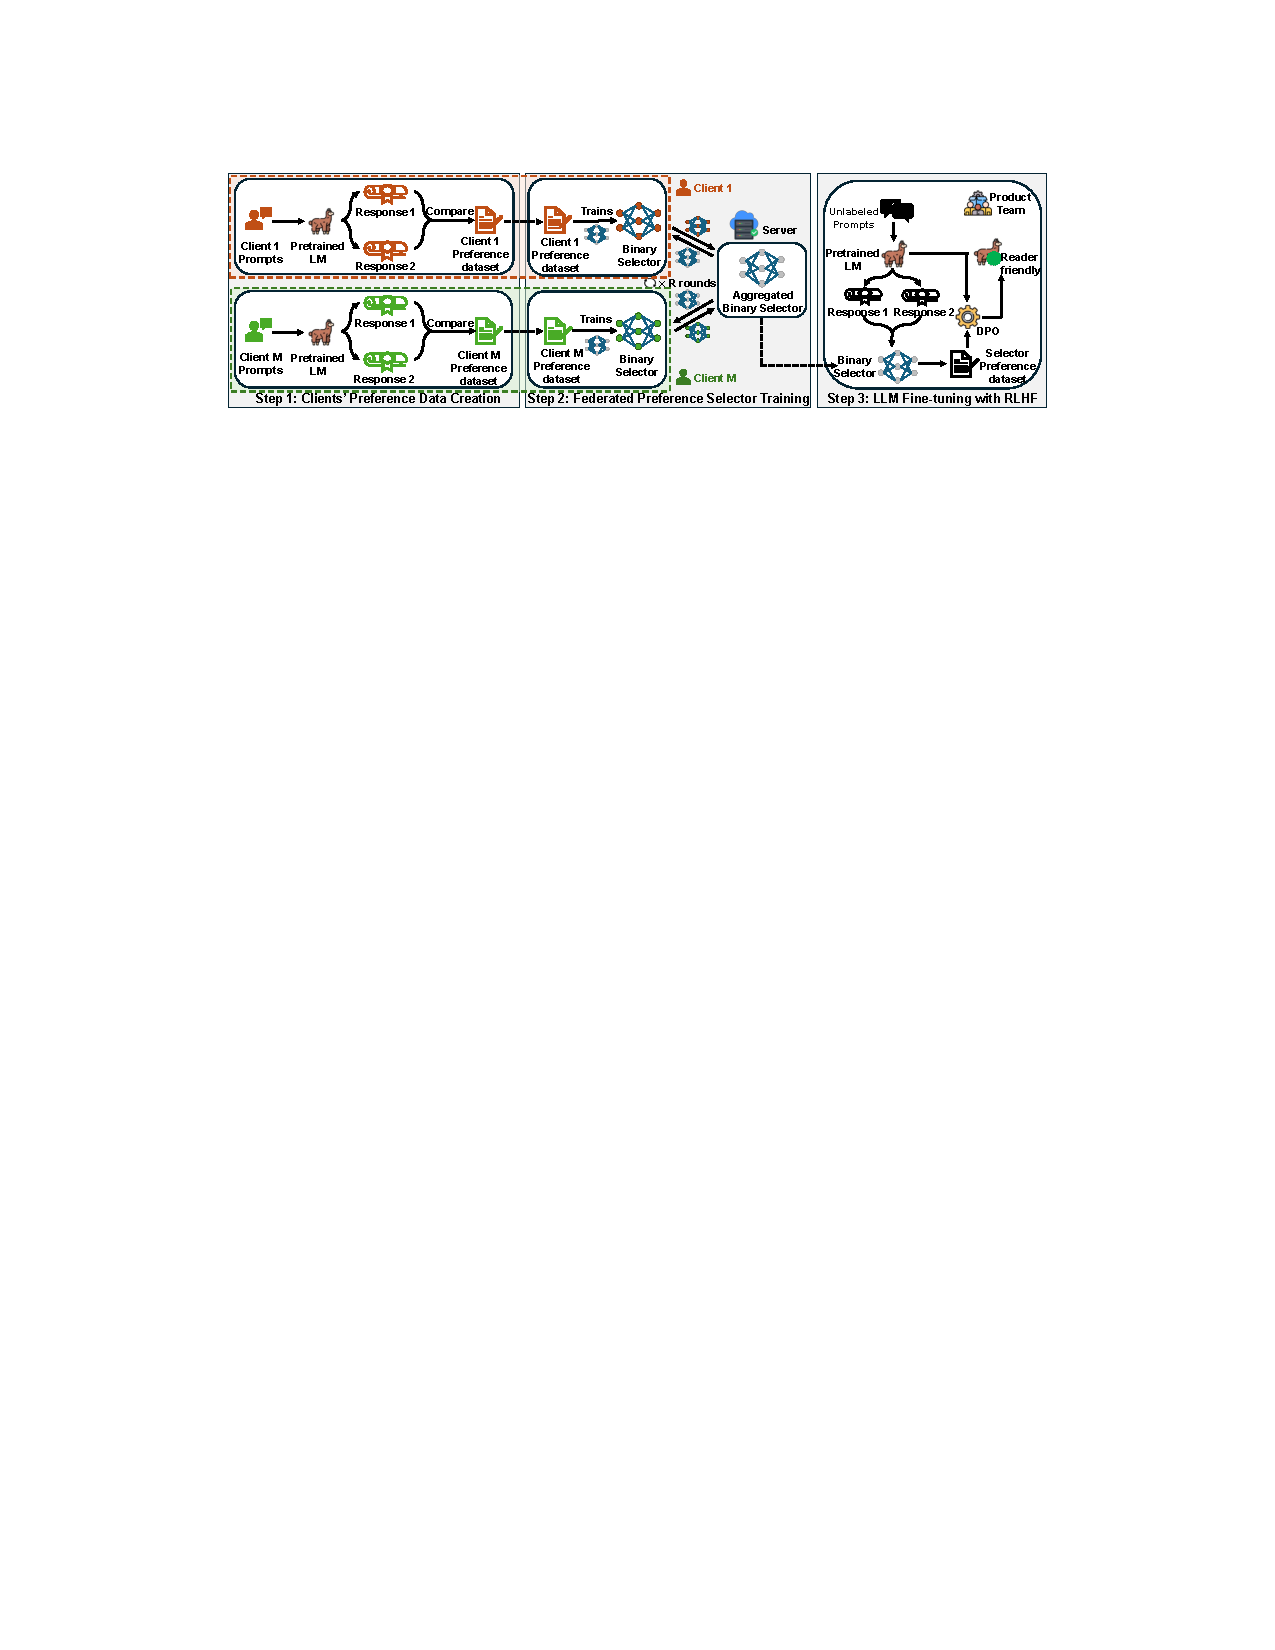
\includegraphics[width=\textwidth]{fedbiscuit-overview.pdf}
  \caption{Overview of FedBiscuit. Figure sourced from \cite{wu2025federatedrlhfaggregatedclient}.}
  \label{fig:overview}
\end{figure*}

\section{Pipeline Overview}
As observed in Figure~\ref{fig:overview}, the pipeline consists of two main training stages. First, clients collaboratively train a binary selector model via federated learning to predict preferences between output pairs (e.g., learning plans). After convergence, the global selector is used to supervise the fine-tuning of the LLM through DPO. For each input, the LLM (e.g., Ol\'e) generates two candidate outputs; the selector picks the preferred one, and DPO updates the LLM accordingly. 

\textsc{FedBiscuit} also supports multi-GPU training via the Hugging Face Accelerate library \cite{accelerate} and integrates well with PEFT methods like LoRA (Low-Rank Adaptation)\cite{hu2021loralowrankadaptationlarge}. LoRA  injects small trainable matrices (<1\% of total model parameters) into frozen model weights, enabling very efficient fine-tuning. This is relevant during the binary selector training phase, where all clients use a shared base model but train distinct adapters. As a result, only the adapters are sent back to the server.

\section{Federated System Design} 
As mentioned earlier, \textsc{FedBiscuit} follows a client-server architecture where, in each communication round, the server distributes the current global model to a subset of selected clients. Each client then fine-tunes the model locally using its own preference data. Once local training is complete, the clients send back their model updates, which the server aggregates to form an updated global model. This iterative process continues until convergence or until a predefined number of rounds has been reached.

\section{Client-Side Operations} 
On the client side, each participant preprocesses their data to construct training samples in the form of preference pairs (i.e., chosen vs. rejected responses to a given prompt). In our adaptation for educational personalization, these preference pairs correspond to selected and discarded learning plans given the student behavioral data and preferences. Local models are trained as a classification task using the cross-entropy loss $\mathcal{L}_{CE}$.

\section{Server-Side Aggregation} 
The central server aggregates model updates without ever accessing raw client data, only model weights or gradients are exchanged. This is enabled by a secure aggregation mechanism, which guarantees that the server can only see the final aggregated result \cite{bonawitz2016practicalsecureaggregationfederated}. The aggregation itself uses FedAvg, a weighted averaging method that accounts for the number of training samples on each client. 

The server also handles client sampling and adapts dynamically to slower or disconnected clients during training.

\section{LLM-as-a-Judge Evaluation} 
To evaluate alignment, \textsc{FedBiscuit} leverages Auto-J, a 13B-parameter generative language model specifically trained to assess other models through natural language critiques. Developed using large-scale user queries and LLM responses, Auto-J achieves competitive performance across 58 real-world evaluation scenarios. In the context of Schol\'e, Auto-J is particularly valuable: it provides an automated, scalable, and interpretable means of assessing how well Ol\'e aligns with learner preferences, without relying on expensive human annotations or black-box evaluators.

\section{Use Case and Limitations} 
\subsubsection{TL;DR Summarization Task} To benchmark alignment performance, \textsc{FedBiscuit} uses the TL;DR summarization task, which consists in generating concise summaries of Reddit posts. This controlled setup helps evaluate preference learning and is later used to estimate the amount of data each client needs in educational settings like for Schol\'e.

\subsubsection{Limitations} 
Despite its strengths, \textsc{FedBiscuit} happens to face some limitations. First, communication overhead remains a bottleneck, especially as the number of clients increases. Second, the system's effectiveness can degrade in the presence of extreme client heterogeneity, both in data quality and hardware capabilities. Finally, the current framework assumes clients have enough data to perform meaningful updates, which may not hold in sparse real-world scenarios. 

In our specific setup, some of these challenges are mitigated. We assume client training occurs on the same server-side machine, removing issues related to hardware variation and network latency. While this setup compromises some of the privacy advantages offered by \textsc{FedBiscuit}, it enables us to establish a strong baseline with full control over the hardware environment. As for data sparsity, this work also introduces methods to generate synthetic data and augment existing datasets, providing a practical solution for low-data scenarios like those found for Schol\'e use case.

